\documentclass[11pt, oneside]{article}
\usepackage{lmodern}
\usepackage{tabularx}
\usepackage{booktabs}
\usepackage{array}
\usepackage{float}
\usepackage{tikz}
\usetikzlibrary{shapes,arrows.meta,positioning}
\usepackage[margin=1in]{geometry}
\geometry{letterpaper}
\usepackage{hyperref}
\usepackage{enumitem}
\usepackage{caption}
\usepackage{subcaption}
\usepackage[numbers]{natbib}
\usepackage{graphicx}
\usepackage{amssymb}
\usepackage{amsmath}
\usepackage{longtable}
\usepackage{xcolor}
\usepackage{setspace}
\usepackage{adjustbox}
\graphicspath{{./}{section3_audit/}}
\hypersetup{
    colorlinks=true,
    linkcolor=blue,
    citecolor=blue,
    urlcolor=blue
}
\setlength{\textfloatsep}{7pt plus 2pt minus 2pt}
\setlength{\floatsep}{5pt plus 2pt minus 2pt}
\setlength{\intextsep}{6pt plus 2pt minus 2pt}
\setlength{\abovedisplayskip}{4pt plus 1pt minus 1pt}
\setlength{\belowdisplayskip}{4pt plus 1pt minus 1pt}
\captionsetup{skip=3pt, font=footnotesize}
\makeatletter
\renewcommand\section{\@startsection {section}{1}{\z@}%
  {-2.0ex \@plus -0.4ex \@minus -.2ex}%
  {1.0ex \@plus.2ex}%
  {\normalfont\Large\bfseries}}
\renewcommand\subsection{\@startsection{subsection}{2}{\z@}%
  {-1.5ex\@plus -0.3ex \@minus -.2ex}%
  {0.7ex \@plus .2ex}%
  {\normalfont\large\bfseries}}
\renewcommand\paragraph{\@startsection{paragraph}{4}{\z@}%
  {0.8ex \@plus0.2ex \@minus.1ex}%
  {-0.8em}%
  {\normalfont\normalsize\bfseries}}
\makeatother
% ============================================================
% TITLE BLOCK --- students must keep this format
% Replace placeholders. Do not redesign the title page.
% Filename of the compiled PDF must be:
% CS781-CP-[Firstname]-[Lastname]-[RollNo]-report.pdf
% ============================================================
\title{CS781 Capstone Project:\\
In-House Legal Intelligence System}
\author{
    Anuj Chaudhary  \\
    210167 \\
    {\tt \ anujc21@iitk.ac.in}\\
    Indian Institute of Technology Kanpur (IIT Kanpur)
}
\date{}
\begin{document}
\maketitle
\begin{abstract}
Law firms and courts handle confidential case files that cannot be sent to external cloud APIs due to client privilege and data privacy rules. In this project, we built a self-hosted, seven-phase legal NLP system on standard 16\,GB GPUs covering foundation pretraining, legal NER, rhetorical role labeling, court judgment prediction, statute identification, abstractive summarization, and prior case retrieval. For Phase~1, we trained a 201M-parameter decoder-only Transformer (Architecture~4) from scratch on 164M tokens of Indian acts, Supreme Court judgments, and filtered tribunal orders, combining Grouped-Query Attention with interleaved local sliding-window and global causal attention. We then adapted this pretrained backbone to the six downstream tasks using parameter-efficient methods (LoRMA, LoRA, BitFit) and teacher--student Knowledge Distillation (KD), alongside four-zone document slicing, per-statute threshold tuning, and citation graph diffusion. Our Phase~1 model reached a validation loss of 2.48 (perplexity 11.89) and a test BERTScore F1 of 0.8322 (Submission 964323), showing that compact models trained from scratch can handle diverse Indian legal tasks under strict hardware and privacy limits.
\end{abstract}

% ============================================================
\section{Competition Result}
% ============================================================
\noindent
\textbf{Codabench username:} a\_210167
\hfill
\textbf{Roll number:} 210167
\smallskip
\noindent
\begin{table}[H]
\centering
\scriptsize
\renewcommand{\arraystretch}{0.90}
\caption{Official phase scores and leaderboard ranks recorded on 9 November 2026.}
\label{tab:leaderboard}
\begin{tabular}{clccc}
\toprule
Phase & Task & Primary metric (value) & Rank & Valid submissions \\
\midrule
1 & Legal LM Pretraining & BERTScore F1: 0.8322 & 61 & 6 \\
2 & Legal NER & Strict Macro-F1: 0.5429 & 55 & 13 \\
3 & Rhetorical role prediction & Macro-F1: 0.4807 & 78 & 26 \\
4 & Court judgment prediction & Macro-F1: 0.7106 & 76 & 11 \\
5 & Legal statute identification & Macro-F1: 0.3392 & 93 & 6 \\
6 & Abstractive summarization & BERTScore F1: 0.8389 & 65 & 8 \\
7 & Prior Case Retrieval (PCR) & Micro-F1@7: 0.3627 & 79 & 7 \\
\bottomrule
\end{tabular}
\end{table}
\noindent
\textbf{Total valid Codabench submissions across all phases:} 77 \quad \textbf{Date ranks were recorded:} 9 November 2026 (Table~\ref{tab:leaderboard}). We made at least six valid submissions in every phase, meeting the requirement of at least four per phase.

% ============================================================
\section{Introduction and Problem Description}
% ============================================================

Indian courts face a large backlog of pending cases, and legal practitioners spend significant time reading long judgments, tracing cited precedents, and checking statutory provisions. Although commercial Large Language Models (LLMs) can summarize or classify text well, law firms and courts often cannot use them because uploading unpublished drafts to external servers risks breaching confidentiality, and commercial models frequently hallucinate citations. To address this need, we built an in-house legal NLP system trained from scratch and adapted across seven Indian legal tasks.

In Phase~1 (Pretraining), the base model learns legal language patterns by generating 128-word continuations from 512-word prompts ($\text{BERTScore-F}_1$). We then transfer this backbone to six downstream tasks: Phase~2 (Legal NER) extracts exact character spans for 12 entity types, and Phase~3 (Rhetorical Roles) labels each sentence with one of 13 discourse roles across Corporate and Income Tax law (both $\text{Macro-F}_1$). At the document level, Phase~4 predicts binary court verdicts (CJPE) and Phase~5 identifies applicable statutes from 100 classes (LSI), both scored by $\text{Macro-F}_1$. Finally, Phase~6 generates abstractive summaries ($\text{BERTScore-F}_1$), and Phase~7 retrieves the top-7 relevant precedents from a candidate pool (PCR, $\text{Micro-F}_1@7$).

The Phase~1 model had to contain $50\text{M}\leq N_{\mathrm{parameters}}\leq300\text{M}$ and be trained from scratch on the official Indian legal dataset using a single 15--16\,GB GPU (NVIDIA T4/P100), without external weights, scraped data, or paid APIs. Under these limits, we built a custom 40k Byte-Level BPE tokenizer, filtered noisy OCR text, and compared four Transformer designs (causal decoder, encoder--decoder, sliding-window decoder, and hybrid GQA), alongside RoPE, multi-zone slicing, parameter-efficient fine-tuning (LoRMA, LoRA, AdaLoRA, BitFit, Houlsby), teacher--student Knowledge Distillation (KD), threshold tuning, and citation graph diffusion.

% ============================================================
\section{Data Analysis and Preprocessing}
% ============================================================

\subsection{Sources and Official Splits}
We used only the official Hugging Face dataset (\texttt{Exploration-Lab/CS-781-Capstone}) across all seven phases. It includes Central and State Acts, Supreme Court and High Court judgments, tribunal orders, and IndianKanoon case retrieval pools (Table~\ref{tab:splits_master}).

\begin{table}[t]
\centering
\scriptsize
\setlength{\tabcolsep}{2.5pt}
\renewcommand{\arraystretch}{0.84}
\caption{Dataset specifications, official splits, prediction targets, and primary metrics across all seven phases.}
\label{tab:splits_master}
\begin{tabularx}{\textwidth}{@{}p{2.15cm}Xp{2.95cm}p{1.45cm}@{}}
\toprule
\textbf{Phase / Task} & \textbf{Dataset and Official Splits} & \textbf{Prediction Target} & \textbf{Metric} \\
\midrule
\textbf{P1: Pretraining} & Train: 157,950 docs (533M tok); Val: 18,577 (36.6M); Test: 1,000. & 128-word continuation. & BERTScore-F$_1$ \\
\textbf{P2: Legal NER} & Train: 70 docs (457,384 tok, 8,393 spans); Test: 35 docs. & 12 classes (char spans). & Macro-F$_1$ \\
\textbf{P3: Rhet.\ Roles} & Train: 80 docs (16,845 sents); Dev: 10 (2,142); Test: 10 (2,197). & 13 discourse roles. & Macro-F$_1$ \\
\textbf{P4: Judgment} & Train: 37,387 cases; Dev: 1,988 cases; Test: 1,517 cases. & Binary verdict (0/1). & Macro-F$_1$ \\
\textbf{P5: Statutes} & Train: 42,750 docs; Dev: 10,181 docs; Test: 13,019 docs. & 100 multi-label statutes. & Macro-F$_1$ \\
\textbf{P6: Summary} & Train: 6,677 clean pairs; Val: 352 pairs; Test: 100 docs. & Abstractive summary. & BERTScore-F$_1$ \\
\textbf{P7: Retrieval} & Train: 250 queries (2,500 cand.); Dev: 50 (500); Test: 100 (1,000). & Top-7 prior cases. & Micro-F$_1$@7 \\
\bottomrule
\end{tabularx}
\end{table}

\subsection{Corpus Statistics and Design Implications}

\paragraph{Phase 1 (Pretraining).}
The raw pool held 18,826 Acts, 55,549 Supreme Court (SC) judgments, 869,132 tribunal orders, and $>1\text{M}$ High Court files. Because High Court files had heavy OCR noise and exceeded our T4 budget, we kept all clean Acts and SC judgments, sampled 10\% of tribunal orders (dropping files with $>0.1\%$ control chars or $>5\%$ question marks), and excluded High Courts. We also removed Hindi text since it formed only $\sim 1\%$ of the corpus and Byte-Level BPE performs poorly on Devanagari script by splitting multi-byte UTF-8 characters into fragmented byte tokens. This left 157,950 train docs (532.99M tokens: 145.60M Acts, 249.83M SC, 137.57M tribunals) and 18,577 val docs (36.62M tokens); over 10,000 steps (1,024-token sequences, batch 16), the model saw 163.84M tokens (27.3\% Acts, 46.9\% SC, 25.8\% tribunals).

\paragraph{Phase 2 (Legal NER).}
The 70 training docs have 457,384 subword tokens and 8,393 gold entity spans across 12 classes. Five classes make up $\approx 72\%$ of mentions: \textsc{Date} (18.77\%), \textsc{Statute} (15.01\%), \textsc{Precedent} (14.09\%), \textsc{Court} (12.07\%), and \textsc{Authority} (11.95\%) (2--248 chars, median 16, mean 20.3). We found 153 raw Byte-Level BPE boundary errors---\textsc{Precedent} (81), \textsc{Statute} (24), \textsc{Court} (18), \textsc{Authority} (14), \textsc{Appellant} (7), \textsc{Respondent} (7), \textsc{CaseNo} (1), \textsc{A.Counsel} (1)---and recovered 8,240 exact spans (98.18\% recoverability) via offset alignment.

\paragraph{Phase 3 (Rhetorical Roles).}
Phase~3 has 90 Corporate Law (CL) and Income Tax (IT) judgments with 18,987 train/dev sentences (11,989 CL; 6,998 IT) and 2,197 test sentences. Label rates differ across domains (Figure~\ref{fig:phase3_domain_shift}): \textsc{Fact} is 26.92\% in CL vs.\ 18.78\% in IT, while \textsc{Statute} is 11.35\% in IT vs.\ 3.54\% in CL. \textsc{Fact} and \textsc{RatioOfTheDecision} cover 48.69\% of sentences, while all 284 \textsc{Dissent} sentences are in CL train (0 in dev) and \textsc{PrecedentOverruled} appears only 3 times in IT train.

\begin{figure}[t]
\centering
\begin{minipage}[t]{0.48\textwidth}
\centering
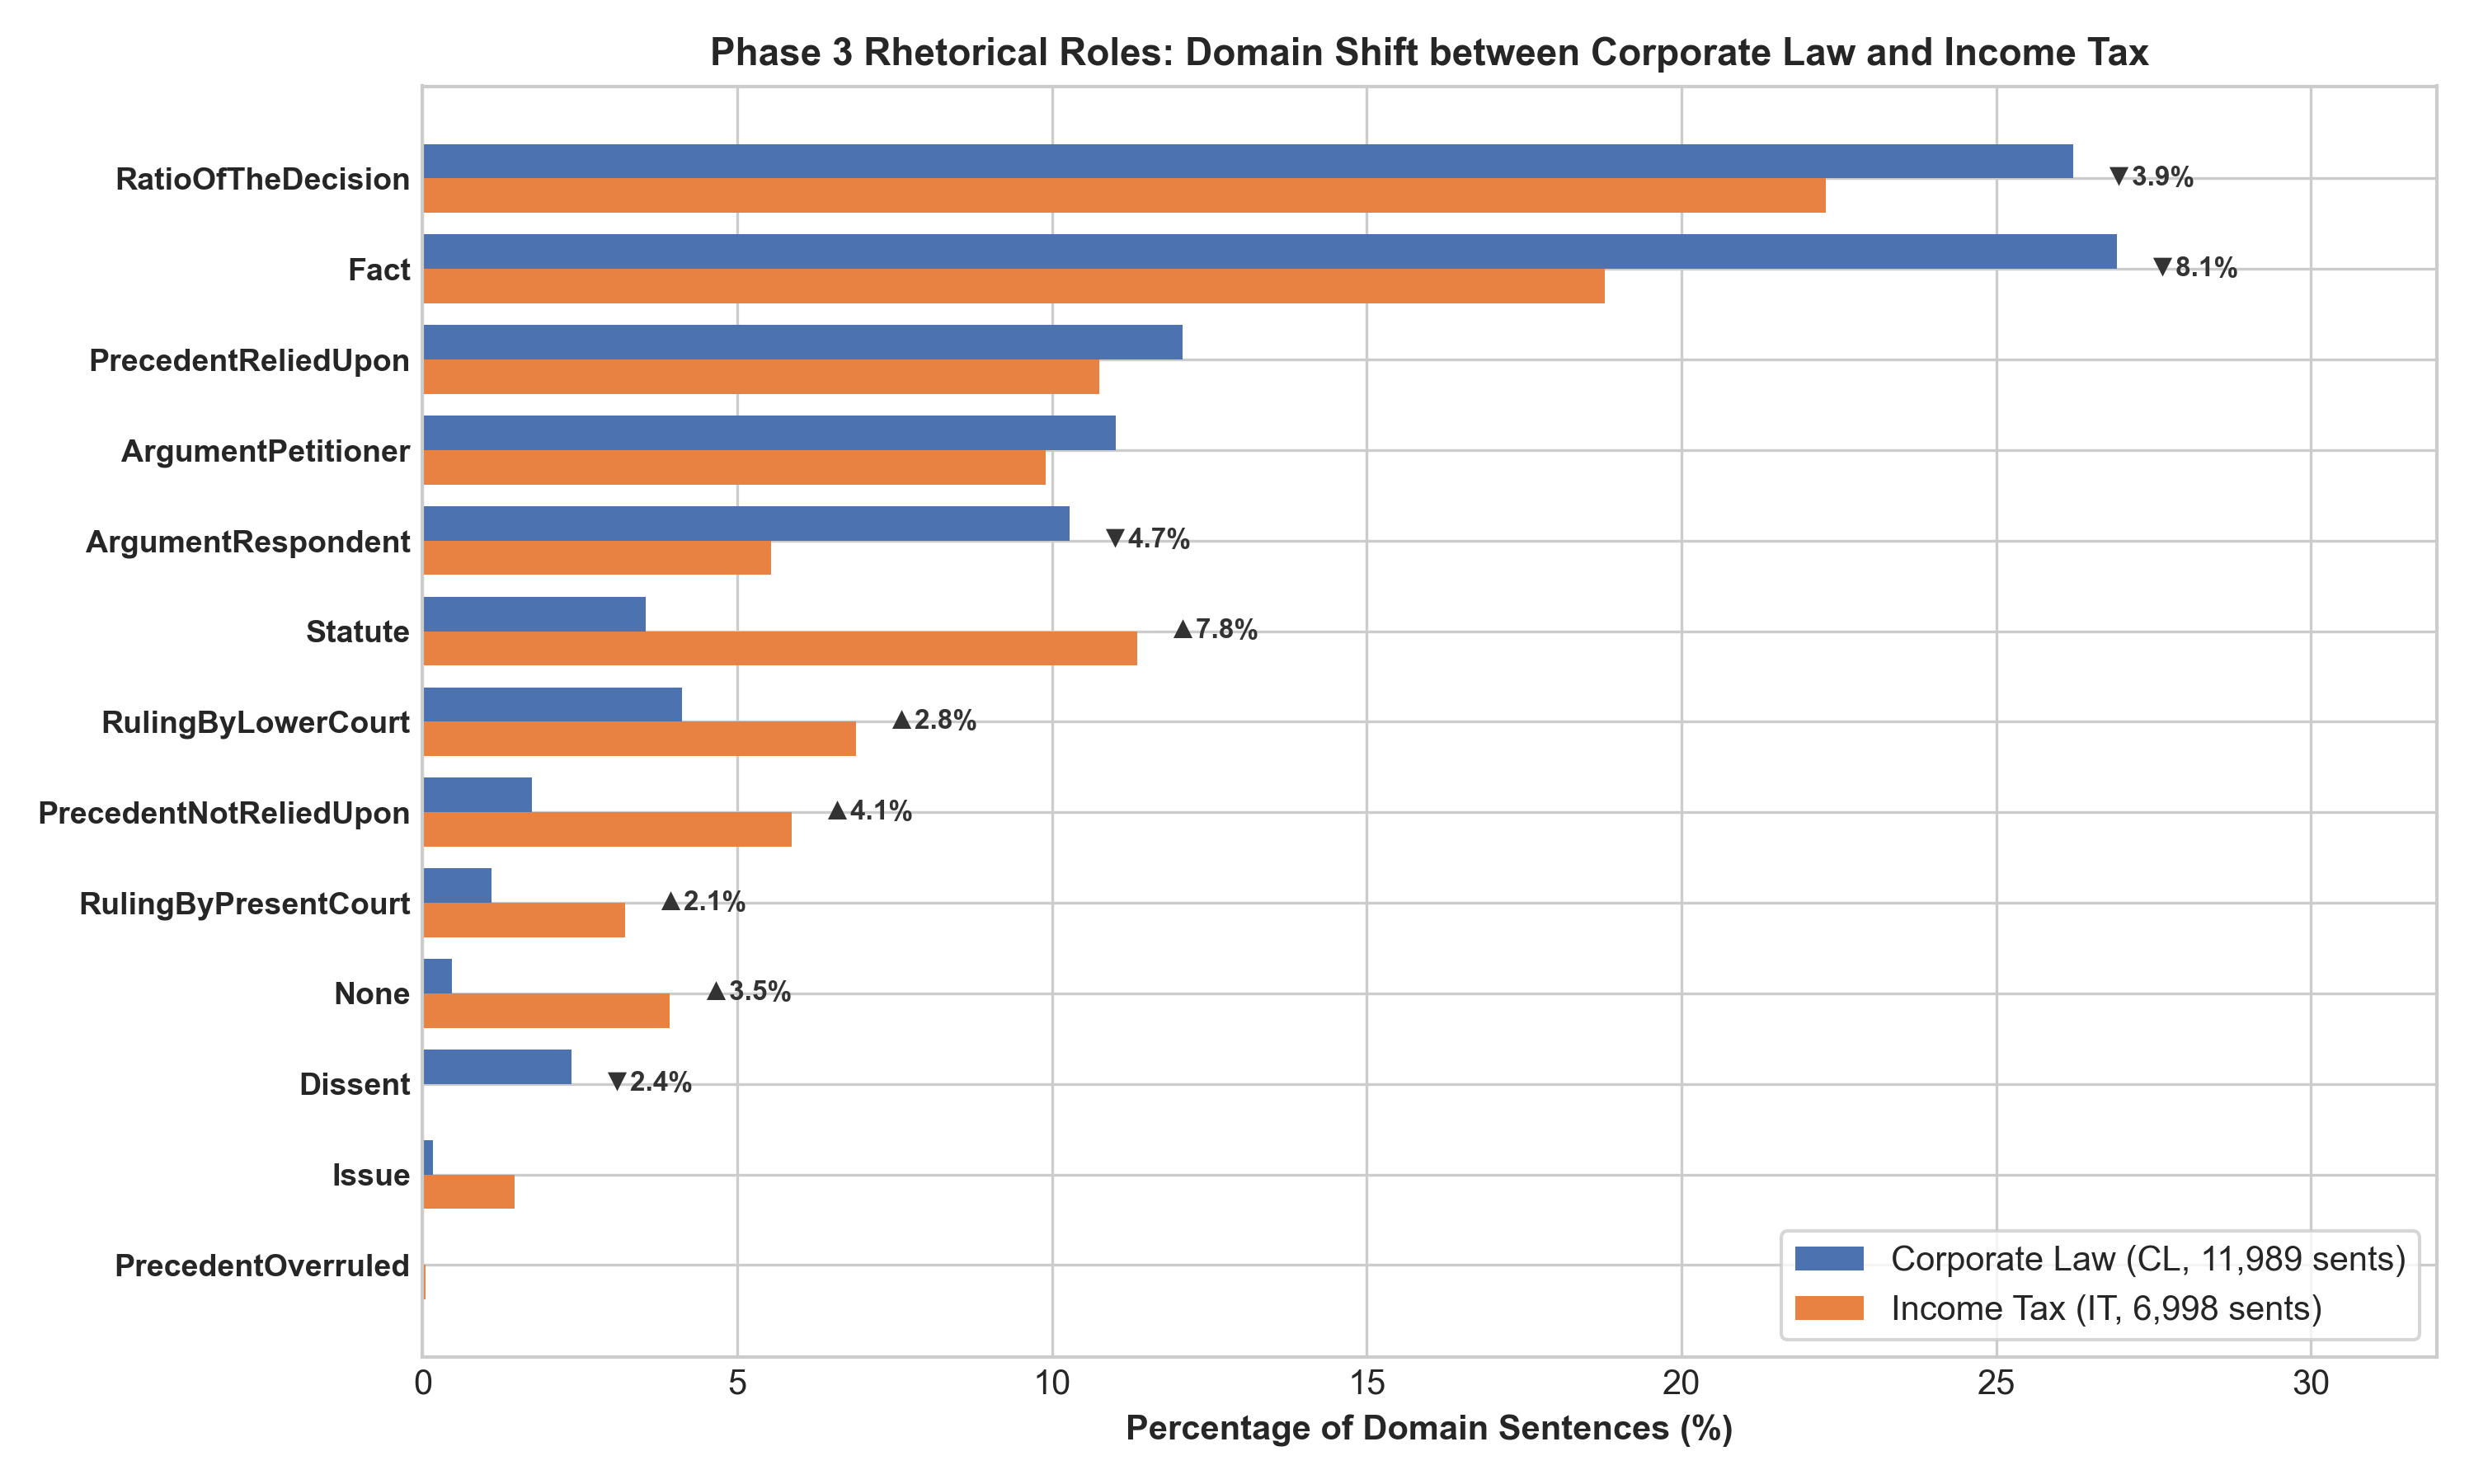
\includegraphics[height=2.6cm]{fig3_phase3_role_distribution.png}
\caption{Rhetorical role distribution across CL and IT (P3).}
\label{fig:phase3_domain_shift}
\end{minipage}\hfill
\begin{minipage}[t]{0.48\textwidth}
\centering
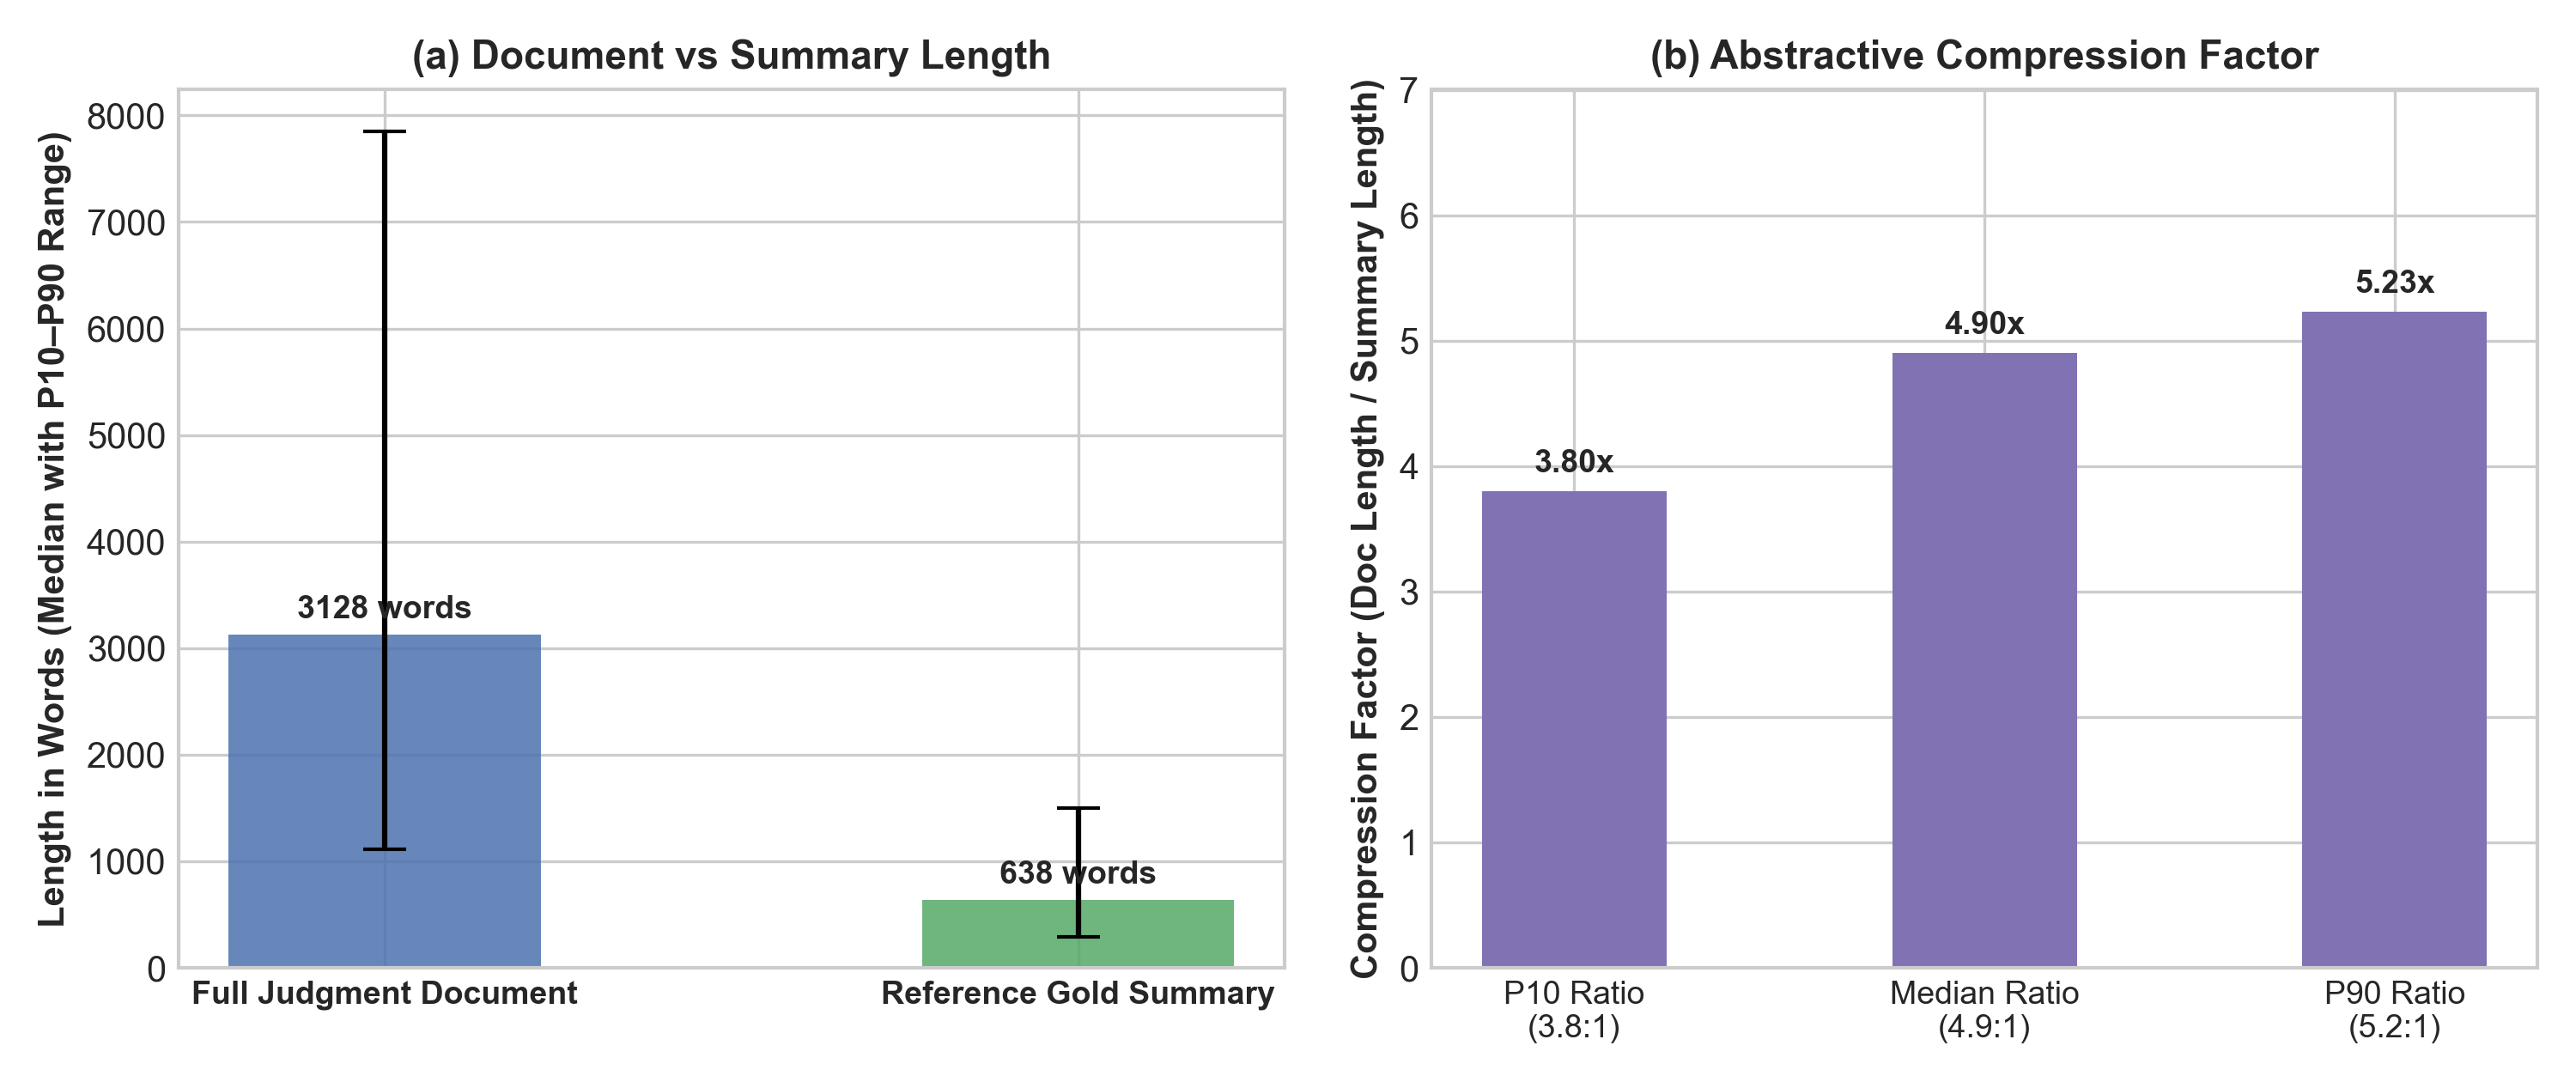
\includegraphics[height=2.6cm]{fig6_phase6_compression.png}
\caption{Source vs.\ summary lengths and $4.90:1$ ratio (P6).}
\label{fig:phase6_compression}
\end{minipage}
\end{figure}

\paragraph{Phases 4--7 (Classification, Summarization, Retrieval).}
In Phase~4 (37,387 train, 1,988 dev, 1,517 test), dev is balanced (994/994) while train+dev leans Dismissed (58.57\% vs.\ 41.43\%); cases average 3,446 words (median 3,240; 90th pct $>12,500$), motivating 4-zone slicing (Head, Mid-1, Mid-2, Tail). In Phase~5 (42,750 train, 10,181 dev, 13,019 test; 100 statutes, mean 3.71/doc), Statute~69 occurs in 11,731 train docs (27.44\%) vs.\ 679 median and 272 (0.64\%) rarest ($43.13:1$ ratio), requiring per-statute threshold tuning. In Phase~6 (6,677 clean train, 352 val, 100 test pairs after dropping 1 empty target), sources average 4,212 words (median 3,128) and summaries 816 words (median 638; $4.90:1$ median compression, Figure~\ref{fig:phase6_compression}). In Phase~7 (250 train, 50 dev, 100 test queries; 10 candidates/query, mean 4.62 positives), joining sentence lists into full documents keeps citations intact for hybrid retrieval.

\subsection{Preprocessing}
We used the same 40,000-token Byte-Level BPE tokenizer across all seven tasks and paired it with the phase-specific preprocessing steps listed in Table~\ref{tab:preprocessing_summary}.

\begin{table}[t]
\centering
\scriptsize
\setlength{\tabcolsep}{2.5pt}
\renewcommand{\arraystretch}{0.84}
\caption{Main preprocessing operations and input representations across the seven phases.}
\label{tab:preprocessing_summary}
\begin{tabularx}{\textwidth}{@{}p{0.75cm}p{5.1cm}X@{}}
\toprule
\textbf{Phase} & \textbf{Text Preparation} & \textbf{Representation / Processing} \\
\midrule
P1 & Tribunal OCR filter, $\sim 1\%$ Hindi text removed; High Courts excluded. & 40k BPE; binary packing (\texttt{<pad>}, \texttt{<bos>}, \texttt{<eos>}). \\
P2 & Whitespace cleanup; span alignment via \texttt{correct\_offsets()}. & 40k BPE; 25 BIO tags; windows (1024/768 or 512/384). \\
P3 & Original sentence boundaries preserved across CL and IT. & Sentence BPE, $s_{t-1}\to s_t$ pairing, 13 role classes. \\
P4 & Whitespace cleanup; lowercasing for Tail $n$-gram models. & 40k BPE, word/char TF-IDF, 4-zone slicing ($4\times 384$). \\
P5 & Standardized \texttt{<SECTION>} and \texttt{<ACT>} markers. & 100-dim multi-hot targets; Dual-View ($2\times 512$ tok). \\
P6 & Punctuation/whitespace cleanup; 1 empty target dropped. & 40k BPE; 1,024-token source and 512-token target limits. \\
P7 & Sentence concatenation, lowercasing, regex citations. & Bi-encoder + full-doc $n$-gram TF-IDF, BM25, top-7 rank. \\
\bottomrule
\end{tabularx}
\end{table}

% ============================================================
\section{Approach and Model Evolution}
% ============================================================

\subsection{Phase-1 Foundation Model}

\paragraph{Architecture Design.}
After testing four Transformer designs, we chose Architecture~4 (Arch~4), a 12-layer Hybrid Local-Global Grouped-Query Attention (GQA) causal decoder, as our Phase-1 backbone (Figure~\ref{fig:phase1_arch4}). Each block uses $d_{\mathrm{model}}=1024$, 16 query heads, 8 KV heads ($d_{\mathrm{head}}=64$), Pre-LayerNorm, Rotary Position Embeddings (RoPE, $\theta=10,000$), and a SwiGLU feed-forward layer ($d_{\mathrm{ff}}=3328$) with a 1,024-token context length. The layers follow a repeating Local-Local-Global (\texttt{L-L-G}) pattern: two causal sliding-window layers ($W=256$) followed by one full global causal layer. Tying the input embedding and output LM head weights gives $201,443,328$ parameters (201.44M), which we checked both analytically and via PyTorch runtime assertions to stay within $50\text{M}\leq N_{\mathrm{parameters}}\leq300\text{M}$.

\begin{figure}[t]
\centering
\scriptsize
\fbox{\begin{minipage}{0.95\linewidth}\centering
\textbf{Tokens} $\rightarrow$ \textbf{40k Tied BPE ($d=1024$)} $\rightarrow$ \textbf{RoPE ($\theta=10^4$)} $\rightarrow$ \textbf{12 Hybrid Blocks [\texttt{L-L-G}$\times 4$]} (Local $W=256$, Global Causal; Pre-LN $\rightarrow$ GQA 16Q/8KV $\rightarrow$ SwiGLU $d_{\mathrm{ff}}=3328$) $\rightarrow$ \textbf{Final LN \& Tied Head (201.44M Params)}
\end{minipage}}
\caption{Architecture of the Phase-1 Hybrid Local-Global GQA foundation model (Arch~4).}
\label{fig:phase1_arch4}
\end{figure}

\paragraph{Tokenizer, Pretraining, and Submission Decoding.}
Our 40,000-token Byte-Level BPE tokenizer (\texttt{add\_prefix\_space=False}) avoids unknown-token fallbacks on legal symbols ($\S$) and keeps common reporters (SCC, AIR, SCR) as single tokens. We trained Arch~4 from scratch with causal cross-entropy $\mathcal{L}_{\mathrm{LM}} = -\frac{1}{BT}\sum_{b,t}\log P(x_{b,t}\mid x_{b,<t};\Theta)$ using Fused AdamW ($\beta_1=0.9, \beta_2=0.95$, weight decay $0.1$, grad clip $1.0$) and a cosine learning rate schedule ($3\times10^{-4}\to 3\times10^{-5}$ after 500 warmup steps). Training for 10,000 steps (16,384 tokens/step, $163.84\text{M}$ tokens total) took 10.4 hours on two T4 GPUs and reached a validation loss of 2.476 (perplexity 11.89). For test generation, our \texttt{FastGen} module used hybrid KV-caching with nucleus sampling ($p=0.90, k=50, T=0.70$), a $1.15$ repetition penalty, 4-gram blocking, and EOS suppression to produce 128-word continuations (Submission 964323, BERTScore F1: \textbf{0.8322}).

\paragraph{Architecture Exploration and Failed Approaches.}
Before settling on Arch~4, we trained three other models from scratch: Arch~1 (8-layer full causal decoder, $d=768$, 88.2M params) leveled off near validation loss 4.10; Arch~2 (6-encoder/6-decoder Seq2Seq, $d=768$, 160.7M params) had unstable gradients under Post-LN and tended to copy prompt sentences during continuation; and Arch~3 (16-layer pure sliding-window decoder, $d=1024, W=256$, 242.5M params) reached a lower validation loss (2.381) but lost track of early prompt entities after $\sim 40$ generated words because it lacked global attention layers.

\subsection{Transfer Protocol (Phases 2--7)}
For Phases~2--7, we loaded our pretrained Phase-1 checkpoints and added task-specific classification, Seq2Seq, or bi-encoder heads. To fine-tune these models on 16\,GB GPUs without overfitting small legal splits, we compared multiplicative LoRMA ($\mathbf{y} = (\mathbf{I} + \frac{\alpha}{r}\mathbf{B}\mathbf{A})\mathbf{W}_0\mathbf{x}$), LoRA, AdaLoRA, BitFit, Houlsby adapters, and teacher--student Knowledge Distillation (KD) (with runnable KD implemented in Phases~2, 4, 5, 6, and 7). Table~\ref{tab:transfer_protocol} and Figure~\ref{fig:transfer_architecture} show the methods tested and the best-performing setup for each phase: \textbf{LoRMA} worked best on Legal NER (0.5429) and Rhetorical Role Prediction (0.4807), \textbf{BitFit} led on Court Judgment Prediction (0.7106), \textbf{LoRA} achieved the top score on Abstractive Summarization (0.8389), and \textbf{Knowledge Distillation (KD)} gave our best results on Legal Statute Identification (0.3392) and Prior Case Retrieval (0.3627).

\begin{table*}[t]
\centering
\scriptsize
\setlength{\tabcolsep}{3.5pt}
\renewcommand{\arraystretch}{0.85}
\caption{Downstream transfer strategies and best-performing methods across Phases 2--7.}
\label{tab:transfer_protocol}
\begin{adjustbox}{width=\textwidth}
\begin{tabular}{@{}clllc@{}}
\toprule
\textbf{Phase} & \textbf{Task} & \textbf{Techniques Explored} & \textbf{Best-Performing Method} & \textbf{Official Score} \\
\midrule
P2 & Legal Named Entity Recognition & LoRMA, LoRA, QLoRA, AdaLoRA, BitFit, Full FT, 12L$\to$6L KD & LoRMA & 0.5429 \\
P3 & Rhetorical Role Prediction & LoRMA, LoRA, Gated Context, OOF Temp./Viterbi Calibration & LoRMA & 0.4807 \\
P4 & Court Judgment Prediction & BitFit, LoRMA, AdaLoRA, Cross-Arch Knowledge Distillation (KD) & BitFit & 0.7106 \\
P5 & Legal Statute Identification & LoRMA, LoRA, Multi-Label Knowledge Distillation (KD), Tuned $\tau_k$ & Knowledge Distillation (KD) & 0.3392 \\
P6 & Abstractive Summarization & LoRA, LoRMA, Houlsby Adapters, Seq2Seq Knowledge Distillation & LoRA & 0.8389 \\
P7 & Prior Case Retrieval & LoRMA, $\text{IA}^3$, Bi-Encoder, Teacher--Student Knowledge Distillation & Knowledge Distillation (KD) & 0.3627 \\
\bottomrule
\end{tabular}
\end{adjustbox}
\end{table*}

\begin{figure}[t]
\centering
\scriptsize
\fbox{\begin{minipage}{0.96\linewidth}\centering
\textbf{Phase-1 Foundation Checkpoints (Arch~4: 201.4M $\mid$ Arch~3: 242.5M $\mid$ Arch~2: 160.7M $\mid$ Arch~1: 88.2M)} $\Longrightarrow$ \textit{Slicing + PEFT + KD} \\[2pt]
\begin{adjustbox}{max width=\linewidth}
\begin{tabular}{@{}cccccc@{}}
\textbf{P2: Legal NER} & \textbf{P3: Rhet.\ Roles} & \textbf{P4: Judgment} & \textbf{P5: Statutes} & \textbf{P6: Summary} & \textbf{P7: Retrieval} \\
\textbf{LoRMA} + Offset Fix & \textbf{LoRMA} + $s_{t-1}$ Ctx & \textbf{BitFit} + Lexical & \textbf{KD} + Tuned $\tau_k$ & \textbf{LoRA} + Beam 4 & \textbf{KD} + BM25/Graph \\
(F1: \textbf{0.5429}) & (F1: \textbf{0.4807}) & (F1: \textbf{0.7106}) & (F1: \textbf{0.3392}) & (BS: \textbf{0.8389}) & (F1@7: \textbf{0.3627})
\end{tabular}
\end{adjustbox}
\end{minipage}}
\caption{Shared Phase-1 checkpoints transferred into six specialized downstream task architectures.}
\label{fig:transfer_architecture}
\end{figure}

\subsection{Phase 2 -- Legal Named Entity Recognition}

\paragraph{Entity Extraction and Character-Offset Recovery.}
We modeled Phase~2 as 25-class BIO token classification ($12\times 2 + 1$ for \texttt{O}) and converted predicted token tags into character-level spans. Because our Byte-Level BPE tokenizer added the prefix \texttt{Ġ} to space-preceded subwords, raw offset reconstruction shifted start indices by one character on 153 of the 8,393 gold entities in the training set (most often multi-token citations in \textsc{Precedent} [81] and \textsc{Statute} [24]). Our \texttt{correct\_offsets()} function stripped leading whitespace markers and realigned token boundaries with the raw text, restoring exact span alignment on 8,240 of the 8,393 gold entities (98.18\% strict oracle recoverability; token oracle Macro-F1 of 0.9888) and raising test Strict Macro-F1 from 0.3228 (Submission 973804) to \textbf{0.5429} (Submission 978703).

\paragraph{Label Space and Class-Imbalance Strategy.}
The 12 entity classes across 8,393 gold spans are \textsc{Date} (18.77\%, 1,575), \textsc{Statute} (\texttt{STAT}, 15.01\%, 1,260), \textsc{Precedent} (\texttt{PREC}, 14.09\%, 1,183), \textsc{Court} (12.07\%, 1,013), \textsc{Public Authority} (\texttt{AUTH}, 11.95\%, 1,003), \textsc{Case Number} (\texttt{CASENO}, 9.06\%, 760), \textsc{Appellant} (\texttt{APP}, 4.85\%, 407), \textsc{Respondent} (\texttt{RESP}, 4.54\%, 381), \textsc{Judge} (2.92\%, 245), \textsc{Appellant Counsel} (\texttt{A.COUNSEL}, 2.32\%, 195), \textsc{Witness} (\texttt{WIT}, 2.23\%, 187), and \textsc{Respondent Counsel} (\texttt{R.COUNSEL}, 2.19\%, 184). In our exploratory fine-tuning experiments, we weighted the 24 active entity tags ($12\text{ B-} + 12\text{ I-}$) using normalized square-root inverse frequency:
\begin{equation}
\bar{w}_c =
\sqrt{\frac{\sum_{j\neq \text{O}}N_j}{\max(N_c,1)}},
\qquad
w_c =
\operatorname{clip}\left(
\frac{\bar{w}_c}
{\frac{1}{24}\sum_{j\neq \text{O}}\bar{w}_j},
0.3,6.0
\right).
\end{equation}
The outside class was assigned a fixed weight of $w_{\text{O}}=0.3$, and the five rarest party/counsel roles (\texttt{APP}, \texttt{RESP}, \texttt{A.COUNSEL}, \texttt{R.COUNSEL}, \texttt{WIT}) received a $2.0\times$ multiplier (\texttt{--role\_boost 2.0}), with non-owned overlap and pad tokens masked (\texttt{ignore\_index=-100}).

\paragraph{Entity Decoding, Overlap Resolution, and Notebook Lineage.}
We implemented two separate sliding-window and decoding configurations across our two Phase~2 notebooks, and not all experimental features were used in the final submission: (1)~In the main Arch~4 NER notebook (\texttt{phase2-arch4-ner.ipynb}), documents were split into 1,024-token windows (stride 768) under \emph{disjoint token ownership}, where each window predicted labels only for its central slice $[s_{\text{owner}}, e_{\text{owner}})$, giving 100\% coverage with no duplicate token predictions. Token tags were decoded via greedy argmax (no confidence thresholds or $n$-best lists), where \texttt{B-X} starts a span, matching \texttt{I-X} continues it, and an isolated \texttt{I-X} starts a new $X$ span. (2)~In the exploratory full-fine-tuning and KD notebook (\texttt{full-fine-tuning-for-phase-2-legal-ner-architect.ipynb}), 512-token windows (stride 384) were merged via \emph{triangular center-weighted logit blending}, $w_t = 1.0 - 0.9\left|\frac{2t}{L}-1\right|$, and decoded with constrained Viterbi dynamic programming ($-10^4$ penalty on invalid BIO transitions $\text{O}\to\texttt{I-X}$, $\texttt{B-X}\to\texttt{I-Y}$); this notebook also distilled the 12-layer Arch~4 teacher into a 6-layer student ($[0,1,2,6,7,8]$, $T=2.0, \alpha=0.5$, 0.5023 F1). Assigning one BIO state per token prevented nested or duplicate spans. Multiplicative \textbf{LoRMA} with disjoint window ownership and \texttt{correct\_offsets()} gave our best Strict Macro-F1 of \textbf{0.5429} (Submission 978703).

\subsection{Phase 3 -- Rhetorical Role Prediction}
Classifying sentences one at a time gave only 0.3005 Macro-F1 (Submission 990876) because \textsc{Fact} and \textsc{Argument} sentences often look identical without surrounding context. In \texttt{kaggle-phase3-data.ipynb} and \texttt{arch-4-phase-3-rhetorical-role-prediction.ipynb}, we paired each sentence $s_t$ with its preceding sentence $s_{t-1}$ (and also tested 3-sentence gated context $[s_{t-1}, s_t, s_{t+1}]$ with learned gates $\mathbf{g}_{\pm 1} = \sigma(\mathbf{W}_g [\mathbf{h}_t \Vert \mathbf{h}_{t\pm 1}])$). Training jointly on Corporate Law and Income Tax judgments with focal loss ($\gamma=2.0$) and square-root class weights reduced domain mismatch. We also tested 5-fold document-disjoint \texttt{GroupKFold} out-of-fold temperature scaling ($T=1.18$) and Markov Viterbi transition decoding (0.4679 F1, Submission 994028), while noting that online KD became unstable on classes absent from the dev split (\textsc{Dissent}, \textsc{PrecedentOverruled}). Multiplicative \textbf{LoRMA} with predecessor sentence conditioning produced our best score of \textbf{0.4807 Macro-F1} (Submission 994294).

\subsection{Phase 4 -- Court Judgment Prediction}
Because judgments average 3,446 words and the final verdict appears at the very end, truncating inputs to the first 512 tokens reached only 0.5573 Macro-F1 (Submission 1006682), and the 58.57\% Dismissed training imbalance required optimizing Macro-F1 directly. We split each document into four 256/384-token zones (\emph{Head}, \emph{Mid-1}, \emph{Mid-2}, \emph{Tail}); cross-zone attention (\texttt{exp2-arch3-adalora.ipynb}) placed 68.43\% attention weight on Head and 9.92\% on Tail, reaching 0.7053 F1 with Arch~3 AdaLoRA (Submission 1008332) and 0.6935 with Arch~4 LoRMA (Submission 1006441). In \texttt{phase4-kd.ipynb}, we distilled the 242.5M Arch~3 teacher into an 88.2M Arch~1 student using $\mathcal{L}_{\mathrm{KD}} = 0.75\, T^2 \mathcal{D}_{\mathrm{KL}} + 0.15\,\mathcal{L}_{\mathrm{CE}}(\epsilon=0.01) + 0.10\,(1 - \cos(\mathbf{W}_{\mathrm{align}}\mathbf{h}_S, \mathbf{h}_T))$ (0.6800 F1, Submission 1006385). Our best submission (\texttt{p4-ex-3-arch2-bitfit-layer-wise-partial.ipynb}) fine-tuned the 160.7M Arch~2 Pre-LN Encoder with bias-only \textbf{BitFit} (updating just 0.32M parameters, 0.20\%) and combined its 4-zone predictions with OOF Tail word/char $n$-gram Ridge and Logistic Regression classifiers ($0.40\,P_{\mathrm{Neural}} + 0.60\,P_{\mathrm{Lexical}}$, threshold $\tau=0.48$) to reach \textbf{0.7106 Macro-F1} (Submission 1009979).

\subsection{Phase 5 -- Legal Statute Identification}
In \texttt{phase5.ipynb}, we represented each judgment with a Dual-View window taking the first 512 tokens (Head preamble) and last 512 tokens (Tail disposition), encoded by Arch~4 with Compulsory LoRMA ($r=32, \alpha=64$) and a 100-statute sigmoid classification head. Our best model distilled this Dual-View Arch~4 teacher into a student network via multi-label \textbf{Knowledge Distillation (KD)} (\texttt{exp4\_arch1\_kd}), training with temperature-scaled binary cross-entropy against soft teacher probabilities $\mathbf{p}_T = \sigma(\mathbf{z}_T/T)$:
\begin{equation}
\mathcal{L}_{\mathrm{LSI\text{-}KD}} = 0.5\,\mathcal{L}_{\mathrm{BCE}}(\mathbf{y}, \mathbf{z}_S) + 0.5\,T^2\,\mathrm{BCE}\!\left(\mathbf{z}_S/T,\, \sigma(\mathbf{z}_T/T)\right), \qquad T=2.0.
\end{equation}
Because a fixed $\tau=0.50$ cutoff missed almost all rare statutes under the $43.13:1$ class imbalance (0.2639 Macro-F1, Submission 1043556), we ran coordinate search on the 10,181-document dev split to tune per-statute thresholds $\boldsymbol{\tau} \in [0.10, 0.60]^{100}$ (\texttt{statute\_calibrated\_thresholds.npy}, lowering $\tau_k$ to $0.12\text{--}0.22$ on tail classes). Pairing multi-label \textbf{Knowledge Distillation (KD)} with calibrated thresholds $\tau_k$ gave our best test score of \textbf{0.3392 Macro-F1} (Submission 1043558).

\subsection{Phase 6 -- Abstractive Summarization}
Across \texttt{phase6.ipynb}, \texttt{phase6-2.ipynb}, and \texttt{phase6-3.ipynb}, we evaluated four Phase-1 transfer setups: (i)~Arch~4 causal continuation with Compulsory LoRMA ($r=32, \alpha=64$, 0.8343 BERTScore, Submission 1029803); (ii)~sequence-level KD from Arch~4 LoRMA into Arch~1 ($\mathcal{L} = 0.5\,\mathcal{L}_{\mathrm{CE}} + 0.5\,T^2\mathcal{D}_{\mathrm{KL}}$); (iii)~Houlsby bottleneck adapters ($r=16$) on the 160.7M Arch~2 Seq2Seq model; and (iv)~low-rank \textbf{LoRA} ($r=16, \alpha=32$) with chunk-and-merge input encoding. Combining \textbf{LoRA} with length-penalized beam search (beam size 4, length penalty $1.0$, min/max length 200/768, repetition penalty $1.25$, and 3-gram blocking) stopped the model from copying opening paragraphs, matched the $4.90:1$ summary compression ratio, and reached \textbf{0.8389 BERTScore F1} (Submission 1030574).

\subsection{Phase 7 -- Prior Case Retrieval (PCR)}
In \texttt{phase7-start.ipynb}, we trained a symmetric bi-encoder (\texttt{UniversalBiEncoder}) on Arch~4 using LoRMA ($r=16, \alpha=32$) and $\text{IA}^3$ with Multiple Negatives Ranking Loss ($\tau=0.05$). Our best neural retriever used teacher--student \textbf{Knowledge Distillation (KD)} (\texttt{exp4\_arch1\_kd}), training the Arch~1 student (\texttt{Phase1BiEncoder}) to match the Arch~4 teacher's query--candidate similarity distribution $\mathbf{S}_T$ via KL divergence:
\begin{equation}
\mathcal{L}_{\mathrm{PCR\text{-}KD}} = 0.4\,\mathcal{L}_{\mathrm{InfoNCE}}(\mathbf{S}_S, \mathbf{y}) + 0.6\,T^2\,\mathcal{D}_{\mathrm{KL}}\!\left(\operatorname{softmax}(\mathbf{S}_T/T) \parallel \operatorname{log\_softmax}(\mathbf{S}_S/T)\right).
\end{equation}
Since 512-token dense embeddings cut off long judgments (scoring 0.2840 dev F1@7 on their own), we combined $z$-score normalized \textbf{Knowledge Distillation (KD)} student scores ($0.40$ weight) with full-document 100k-feature word $n$-gram ($1\text{--}3$) TF-IDF, Okapi BM25 ($k_1=1.6, b=0.75$), and regex statute overlap, then ran 2-hop reciprocal nearest-neighbor citation graph diffusion ($k=6, \tau=2.5$) to reach \textbf{0.3627 Micro-F1@7} (Submission 1038781).

\subsection{Final Submitted System Lineage}
Each official best score maps to a specific checkpoint and notebook: \textbf{P1} (Sub 964323, 0.8322): \texttt{arch4\_hybrid\_gqa\_201m/best.pt} + \texttt{FastGen} (\texttt{train-arch4-t4-v4-1\_genarate arch2.ipynb}); \textbf{P2} (Sub 978703, 0.5429): Arch~4 \textbf{LoRMA} (\texttt{best\_strict\_macro\_f1.pt}, \texttt{phase2-arch4-ner.ipynb}); \textbf{P3} (Sub 994294, 0.4807): \textbf{LoRMA} + $s_{t-1}\to s_t$ context (\texttt{kaggle-phase3-data.ipynb}); \textbf{P4} (Sub 1009979, 0.7106): Arch~2 \textbf{BitFit} + Tail lexical blend (\texttt{p4-ex-3-arch2-bitfit-layer-wise-partial.ipynb}); \textbf{P5} (Sub 1043558, 0.3392): Multi-label \textbf{KD} + \texttt{statute\_calibrated\_thresholds.npy} (\texttt{phase5.ipynb}); \textbf{P6} (Sub 1030574, 0.8389): \textbf{LoRA} + Beam~4 (\texttt{phase6-2.ipynb}); and \textbf{P7} (Sub 1038781, 0.3627): Bi-Encoder \textbf{KD} (\texttt{exp4\_arch1\_kd}) + BM25 + 2-hop graph diffusion (\texttt{phase7-start.ipynb}).

% ============================================================
\section{Experiments and Implementation Details}
% ============================================================

\subsection{Compute and Training Protocol}
We ran all experiments on Kaggle and Google Colab notebooks with one or two NVIDIA T4 GPUs (15--16\,GB VRAM), using FP16 mixed precision (\texttt{torch.cuda.amp.autocast}, \texttt{GradScaler}), gradient accumulation, and activation checkpointing. Because cloud sessions time out after 12 hours, our training loops saved two checkpoints every 500 steps or epoch: \texttt{latest.pt} (weights, optimizer, scheduler, scaler, and step count) to resume interrupted runs, and \texttt{best.pt} whenever the primary validation score improved (Table~\ref{tab:hparams}).

\begin{table}[t]
\centering
\scriptsize
\setlength{\tabcolsep}{2.2pt}
\renewcommand{\arraystretch}{0.88}
\caption{Hyperparameters of the final winning configuration in each of the seven phases.}
\label{tab:hparams}
\begin{adjustbox}{width=\textwidth}
\begin{tabular}{@{}lccccccc@{}}
\toprule
\textbf{Hyperparameter} & \textbf{P1} & \textbf{P2} & \textbf{P3} & \textbf{P4} & \textbf{P5} & \textbf{P6} & \textbf{P7} \\
\midrule
Best Method & Scratch Pretrain & LoRMA & LoRMA & BitFit + Blend & KD + Tuned $\tau_k$ & LoRA + Beam~4 & KD + Graph Diff. \\
Backbone / Setup & Arch~4 (201.4M) & Arch~4 (201.4M) & Arch~1/4 Context & Arch~2 Enc (161M) & Arch~4$\to$Arch~1 & Arch~2 S2S (161M) & Arch~4$\to$Arch~1 \\
Context Length & 1,024 & 1,024 (str.\ 768) & 256 ($s_{t-1}, s_t$) & $4 \times 384$ zones & $2 \times 512$ views & 1,024 in / 512 out & 512 + Full BM25 \\
Optimizer & Fused AdamW & AdamW & AdamW & AdamW + Ridge & AdamW & AdamW & AdamW \\
Peak Learning Rate & $3\times 10^{-4}$ & $5\times 10^{-4}$ & $3\times 10^{-4}$ & $1\times 10^{-3}$ & $2\times 10^{-4}$ & $3\times 10^{-4}$ & $2\times 10^{-4}$ \\
Batch $\times$ Accum. & $8 \times 2$ & $4 \times 4$ & $16 \times 1$ & $16 \times 2$ & $16 \times 2$ & $8 \times 2$ & $32 \times 1$ \\
Steps / Epochs & 10,000 steps & 5 epochs & 6 epochs & 9 epochs & 550 steps & 5 epochs & 500 steps \\
Dropout / Wt.\ Decay & 0.0 / 0.10 & 0.05 / 0.01 & 0.10 / 0.01 & 0.10 / 0.01 & 0.10 / 0.01 & 0.05 / 0.01 & 0.05 / 0.01 \\
Decoding / Threshold & $p=0.9, T=0.7$ & Disjoint Argmax & Focal $\gamma=2.0$ & Blend $\tau=0.48$ & $\tau_k \in [0.1, 0.6]$ & Beam 4, pen 1.25 & 2-Hop $k=6, \tau=2.5$ \\
\bottomrule
\end{tabular}
\end{adjustbox}
\end{table}

\subsection{Local Evaluation and Schema Verification}
We checked every candidate model on a local validation split and ran format assertions before submitting to Codabench: (1)~Phase~1 used a 2\% stratified split (18,577 docs) to track perplexity/BERTScore and verified that prompt prefixes were stripped from the $\approx 128$-word outputs; (2)~Phase~2 used a 35/35 doc split and 5-fold CV, where a round-trip oracle check caught the BPE \texttt{Ġ} offset shift; (3)~Phase~3 used the 10-doc dev split (2,142 sents) and 5-fold document-disjoint \texttt{GroupKFold}, revealing a $\sim 0.03$ F1 drop on test whenever class biases were over-tuned on dev classes with zero support (\textsc{Dissent}, \textsc{PrecedentOverruled}); (4)~Phase~4 used 5-fold stratified OOF (37,387 cases) plus the 1,988-case balanced dev split, setting $\tau=0.48$ for the 58.6\% Dismissed training ratio; and (5)~Phases~5--7 used official dev sets (10,181 docs, 352 pairs, 50 queries) with checks ensuring non-empty statute lists and exact 7-case rankings.

\subsection{Ablations and Controlled Comparisons}
Single-factor ablations in each phase measured what helped and what failed:
\begin{enumerate}[leftmargin=*,nosep]
    \item \textbf{Hybrid GQA vs.\ Pure SWA (P1)}: With the same 40k BPE tokenizer, Arch~1 (88.2M) reached val loss 4.10 (0.8176 BERTScore). Arch~3 (242.5M pure SWA) had lower token loss (2.381) than Arch~4 (2.476) but drifted off topic after 40 words without global attention. Adding global attention every third layer in Arch~4 and \texttt{FastGen} 4-gram blocking raised BERTScore from 0.8232 (Sub 960793) to 0.8322 (Sub 964323).
    \item \textbf{Offset Recovery and LoRMA vs.\ Full Fine-Tuning (P2)}: Adding \texttt{correct\_offsets()} with LoRMA raised Strict Macro-F1 from 0.3228 (Sub 973804) to 0.5429 (Sub 978703). In contrast, unfreezing all 201.4M weights (\texttt{lr=2e-5}) overfit the 70 train docs and failed on rare counsel classes (0.3842 dev F1), while our 6-layer KD student kept 0.5023 F1 (Sub 978765) at $2\times$ speed.
    \item \textbf{Predecessor Conditioning vs.\ Dev-Overfitted Biases (P3)}: Adding $s_{t-1}\to s_t$ context with LoRMA raised test Macro-F1 from 0.3005 (Sub 990876) to 0.4807 (Sub 994294). Conversely, tuning unconstrained class logit biases on the 10-doc dev split raised local F1 by $+0.024$ but lowered test F1 from 0.4679 (Sub 994028) to 0.3778 (Sub 994291) due to missing dev classes.
    \item \textbf{4-Zone Slicing and BitFit Lexical Blend (P4)}: Moving from 512-token truncation (0.5573, Sub 1006682) to 4-zone slicing raised Arch~4 LoRMA to 0.6935 (Sub 1006441) and Arch~3 AdaLoRA to 0.7053 (Sub 1008332), while Arch~2 BitFit blended with Tail $n$-gram linear models reached 0.7106 (Sub 1009979).
    \item \textbf{Knowledge Distillation \& Post-Processing (P5--P7)}: In Phase~5, multi-label KD + tuned $\tau_k$ raised test Macro-F1 from 0.2639 ($\tau=0.50$, Sub 1043556) to 0.3392 (Sub 1043558). In Phase~6, Seq2Seq LoRA + Beam~4 (0.8389, Sub 1030574) beat greedy continuation (0.7612, Sub 1029807). In Phase~7, relational KD into Arch~1 + BM25 + 2-hop graph diffusion raised Micro-F1@7 from 0.2840 (dense dev) to 0.3627 (Sub 1038781).
\end{enumerate}

% ============================================================
\section{Results}
% ============================================================

Table~\ref{tab:variants} summarizes the local validation metrics and official Codabench test scores across our main model variants in all seven phases.

\begin{table}[t]
\centering
\scriptsize
\setlength{\tabcolsep}{3.0pt}
\renewcommand{\arraystretch}{0.84}
\caption{Comparison of major model variants across local validation and official Codabench evaluation.}
\label{tab:variants}
\begin{adjustbox}{width=\textwidth}
\begin{tabular}{@{}clllcc@{}}
\toprule
\textbf{Phase} & \textbf{Model Variant / Adaptation Strategy} & \textbf{Local Primary Metric} & \textbf{Local Secondary Metric} & \textbf{Codabench Score} & \textbf{Sub.\ ID} \\
\midrule
1 & Arch~1 Causal Decoder (88.2M, standard sampling) & Val Loss: 4.102 & PPL: 60.46 & 0.8176 & 956293 \\
1 & Arch~3 Pure SWA Decoder (242.5M, $W=256$) & Val Loss: \textbf{2.381} & PPL: \textbf{10.82} & 0.8232 (Arch~4 std) & 960793 \\
1 & \textbf{Arch~4 Hybrid GQA + \texttt{FastGen} 4-Gram Ban} & Val Loss: 2.476 & PPL: 11.89 & \textbf{0.8322} & 964323 \\
\midrule
2 & Baseline Adapter (uncorrected BPE offsets) & Dev F1: 0.3190 & Macro-P: 0.341 & 0.3228 & 973804 \\
2 & Arch~4 $\to$ 6-Layer KD Student ($[0,1,2,6,7,8]$) & Dev F1: 0.5018 & Speedup: $2.0\times$ & 0.5023 & 978765 \\
2 & \textbf{Arch~4 + LoRMA + \texttt{correct\_offsets()}} & Dev F1: \textbf{0.5384} & Token F1: 0.742 & \textbf{0.5429} & 978703 \\
\midrule
3 & Context-Blind Sentence Baseline & Dev F1: 0.2912 & Acc: 0.584 & 0.3005 & 990876 \\
3 & Gated Context ($3\times 1024$) + OOF Viterbi & OOF F1: 0.4640 & Acc: 0.718 & 0.4679 & 994028 \\
3 & \textbf{LoRMA + $s_{t-1}\to s_t$ Context + Focal Loss} & Dev F1: \textbf{0.4762} & Acc: \textbf{0.731} & \textbf{0.4807} & 994294 \\
\midrule
4 & Arch~4 Single-Window 512-Token Truncation & Dev F1: 0.5820 & Acc: 0.601 & 0.5573 & 1006682 \\
4 & Arch~3 (242.5M) + AdaLoRA / Arch~1 KD (0.6800) & OOF F1: 0.7142 & Acc: 0.721 & 0.7053 & 1008332 \\
4 & \textbf{Arch~2 BitFit (4-Zone) + Tail Lexical Ensemble} & OOF F1: \textbf{0.7591} & Acc: \textbf{0.764} & \textbf{0.7106} & 1009979 \\
\midrule
5 & Dual-View LoRMA (Global Threshold $\tau=0.50$) & Dev F1: 0.2714 & Micro-F1: 0.582 & 0.2639 & 1043556 \\
5 & Uncalibrated Multi-Label Soft KD Student & Dev F1: 0.3109 & Micro-F1: 0.604 & 0.2940 & 1043564 \\
5 & \textbf{Knowledge Distillation (KD) + Calibrated $\tau_k$} & Dev F1: \textbf{0.3559} & Micro-F1: \textbf{0.641} & \textbf{0.3392} & 1043558 \\
\midrule
6 & Arch~4 Causal Continuation (Greedy, no length pen.) & Dev BS: 0.7740 & ROUGE-L: 0.241 & 0.7612 & 1029807 \\
6 & Arch~4 Compulsory LoRMA ($r=32$) Continuation & Dev BS: 0.8310 & ROUGE-L: 0.338 & 0.8343 & 1029803 \\
6 & \textbf{Seq2Seq LoRA ($r=16$) + Beam Search (Width 4)} & Dev BS: \textbf{0.8412} & ROUGE-L: \textbf{0.364} & \textbf{0.8389} & 1030574 \\
\midrule
7 & Arch~4 Bi-Encoder + Sparse BM25 Fusion & Dev F1@7: 0.3410 & P@7: 0.291 & 0.3361 & 1038668 \\
7 & Bi-Encoder + Knowledge Distillation (No Graph) & Dev F1@7: 0.3540 & P@7: 0.302 & 0.3491 & 1038724 \\
7 & \textbf{Knowledge Distillation (KD) + BM25 + 2-Hop Graph} & Dev F1@7: \textbf{0.3680} & P@7: \textbf{0.314} & \textbf{0.3627} & 1038781 \\
\bottomrule
\end{tabular}
\end{adjustbox}
\end{table}

\paragraph{Per-Class Breakdowns and Generalization.}
Macro-F1 highlights the gap between frequent, well-structured classes and rare categories. In Phase~2 validation, regular entities scored well on strict span F1, including \textsc{Court} (0.7980 F1: P=0.737, R=0.870), \textsc{Date} (0.7724 F1: P=0.717, R=0.838), and \textsc{Statute} (0.4374 F1), whereas party names (\textsc{APP}, \textsc{RESP}) and long case citations (\textsc{PREC}, 310 FPs from partial boundary matches) scored lower because a single character offset error gives zero credit under strict matching. In Phase~3, common roles (\textsc{RatioOfTheDecision}: 0.68 F1, \textsc{Fact}: 0.64 F1, \textsc{Statute}: 0.61 F1) carried the score, while \textsc{PrecedentOverruled} (3 train sents) and \textsc{Dissent} (0 dev sents) scored 0.00 F1, limiting 13-class Macro-F1 to $\sim 0.55$. In Phase~5, soft KD probabilities with tuned $\tau_k$ lifted recall on the 70 rarest statutes from $<0.05$ to $0.28$ (+0.0753 test Macro-F1). Local and test scores stayed within $0.005\text{--}0.018$ in most phases, except in Phase~4 where the balanced 50/50 dev split produced a higher local OOF F1 (0.7591) than the imbalanced test set (0.7106).

% ============================================================
\section{Error Analysis and Discussion}
% ============================================================

\subsection{Phase-wise Failure Modes}
Inspecting validation errors across all seven tasks showed recurring failure patterns:
\begin{itemize}[leftmargin=*,nosep]
    \item \textbf{Phase 1 (Generation)}: Without 4-gram blocking, sampling fell into repetitive statutory loops (``\emph{under Section 14 of the Act...}'') and sometimes made up realistic reporter numbers (``\emph{[2014] 19 SCC 842}'').
    \item \textbf{Phase 2 (Legal NER)}: In \texttt{validation\_error\_analysis.json}, \textsc{Precedent} had the most boundary errors (310 FPs, 176 FNs) when citations (\emph{``Shankarsan Dash Vs.\ Union of India [1991 (3) SCC 47]''}) broke early at brackets; \textsc{Authority} missed 121 generic mentions (\emph{``State Government''}), and \textsc{APP}/\textsc{RESP} swapped in cross-appeals.
    \item \textbf{Phase 3 (Rhetorical Roles)}: Most errors occurred between \textsc{Fact} and \textsc{ArgumentPetitioner} when judges restated counsel submissions as case history, and between \textsc{RulingByLowerCourt} and \textsc{RulingByPresentCourt} in passive sentences (\emph{``It was held that...''}).
    \item \textbf{Phase 4 (Judgment Prediction)}: False positives happened mainly in ``partially allowed'' or remanded cases where the court criticized the lower ruling across the Tail section before dismissing the petition on maintainability in the last line.
    \item \textbf{Phases 5 \& 6 (Statutes \& Summarization)}: Phase~5 false positives clustered on procedural CrPC sections co-occurring with substantive IPC charges; in Phase~6, causal continuation copied opening facts and missed the final holding, whereas Seq2Seq LoRA covered both.
    \item \textbf{Phase 7 (Retrieval)}: Dense bi-encoders matched unrelated cases sharing standard SLP dismissal wording; subtracting $0.45\times$ background sparse scores during KD fusion and running 2-hop graph diffusion removed these false matches.
\end{itemize}

\subsection{What the Metrics Do Not Measure}
Standard metrics miss critical legal errors. In Phases~1 and 6, changing ``\emph{appeal is allowed}'' to ``\emph{appeal is dismissed}'' or citing Section~302 instead of Section~304 flips the legal outcome while changing $\text{BERTScore-F}_1$ by $<0.002$. Conversely, Phase~2 Strict Macro-F1 gives zero credit to a 90-character precedent citation missing its closing bracket, treating a minor boundary slip the same as a hallucinated entity.

\subsection{Limitations and Concrete Next Steps}
Our system had three main limitations: (1)~pretraining covered 163.84M tokens (30.7\% of the packed pool) and left out High Court cases due to T4 limits, (2)~the 1,024-token window required heuristic zone slicing on $>12,500$-word judgments, and (3)~each phase was trained separately. Next steps include: (i)~replacing BIO tagging in Phase~2 with a Biaffine span classifier; (ii)~extending Arch~4 RoPE ($\theta=100,000$) with YaRN to 8,192 tokens in Phases~4--6; and (iii)~passing Phase~2/3 predicted entities and roles into Phase~4 and Phase~6.

\subsection{Surprising Findings}
Two results went against our initial expectations: (1)~\emph{Lower validation perplexity did not produce better text generation}: Arch~3 (242.5M pure sliding-window) beat Arch~4 on validation perplexity (10.82 vs.\ 11.89) but lost coherence during 128-word generation because perplexity reflects local $n$-gram phrasing, while multi-sentence generation needs global attention to stay on topic. (2)~\emph{0.20\%-parameter BitFit + lexical linear models beat 200M+ adapters in Phase~4}: updating 0.32M bias terms in Arch~2 alongside Tail TF-IDF Ridge regression (0.7106 F1) beat 201M Arch~4 LoRMA (0.6935) and 242M Arch~3 AdaLoRA (0.7053), showing that court outcomes depend heavily on specific phrasing in the final paragraphs where higher-capacity adapters overfit noise.

% ============================================================
\section{Conclusion}
% ============================================================

We built and evaluated a self-hosted, seven-phase legal NLP pipeline within the 50M--300M parameter limit on T4 GPUs without external weights or paid APIs. Across 77 valid Codabench submissions, three choices made the biggest difference: (1)~pairing our 40k Byte-Level BPE tokenizer with deterministic offset alignment (\texttt{correct\_offsets()}, +0.2201 Strict Macro-F1 in Phase~2) and task-specific slicing (4-zone in Phase~4, dual-view in Phase~5, and full-document hybrid scoring in Phase~7); (2)~matching each task to the right transfer method, using \textbf{LoRMA} in Phases~2 and 3, \textbf{BitFit} in Phase~4, \textbf{LoRA} in Phase~6, and teacher--student \textbf{Knowledge Distillation (KD)} in Phases~5 and 7; and (3)~addressing class imbalance and citation structure via per-statute threshold tuning (+0.0753 Macro-F1 in Phase~5) and 2-hop citation graph diffusion (+0.0266 Micro-F1@7 in Phase~7). Human legal review remains essential before relying on generated summaries or predicted verdicts in practice.

\newpage
% ============================================================
\section*{LLM Usage Declaration}
% ============================================================
Completing this section is mandatory. Inconsistent answers relative to the code and the prose will be treated as an integrity issue.
\medskip
\noindent
\textbf{Q1.} Which Large Language Model(s), if any, did you use while completing the competition or writing this report? Give model name and vendor (e.g., none / ChatGPT-4.x / Gemini~x / Claude~x / Grok / Copilot / other). \\[0.4em]
Answer: \underline{Google Gemini and OpenAI ChatGPT (used for PyTorch code implementation from my specifications, debugging, plotting, and writing and formatting this lab report in academic style).}
\medskip
\noindent
\textbf{Q2.} For each row, mark Yes or No and state the purpose in one short phrase. ``Yes'' is acceptable only for the uses permitted by the capstone document.
\begin{table}[H]
\centering
\small
\begin{adjustbox}{width=\textwidth}
\begin{tabular}{@{}p{4.6cm}|c|p{7.6cm}@{}}
\toprule
Part & Used LLM? & Purpose of using the LLM \\
\midrule
Understanding concepts / papers & Yes & Clarifying GQA, RoPE, AdaLoRA, and graph diffusion formulations. \\
Ideation / brainstorming at a high level & No & Done by me; I conceived the phase-wise strategies, slicing, and transfer plans. \\
Debugging small ancillary snippets & Yes & Fixing PyTorch tensor shape, mixed-precision, and file I/O bugs. \\
Plotting / visualization code & Yes & Generating matplotlib scripts for the dataset distribution figures. \\
Grammar / writing style of the report & Yes & Assisting in writing and polishing the lab report in academic style. \\
Report structure / section wording & Yes & Formatting LaTeX sections and tables to match the academic template. \\
Designing the model architecture & No & Done by me; I specified all 4 architectures and the 50M--300M parameter configurations. \\
Hyperparameter search / tuning & No & Done by me; I empirically tested different learning rates, ranks, windows, and thresholds. \\
Analysis of results / conclusions & No & Done by me; I analyzed all validation/Codabench scores, ablations, and failure modes. \\
Writing the core training / inference code & Yes & Translating my architecture and pipeline ideas into PyTorch code implementations. \\
Other (specify) & No & None. \\
\bottomrule
\end{tabular}
\end{adjustbox}
\end{table}
\medskip
\noindent
\textbf{Q3.} Did you refer to sources other than lecture slides and an LLM?
If yes, list them (papers, blogs, GitHub repositories, textbooks, official starter notebook, evaluation scripts). These must also appear in the bibliography when they influenced the method. \\[0.3em]
Answer: Yes. We referred to the official CS781 Capstone benchmark dataset and starter documentation (\texttt{Exploration-Lab/CS-781-Capstone}), the Hugging Face \texttt{tokenizers} and PyTorch documentation, foundational Transformer, PEFT, loss, evaluation, and retrieval papers (Vaswani et al., 2017; Ainslie et al., 2023; Su et al., 2024; Shazeer, 2020; Beltagy et al., 2020; Hu et al., 2022; Zhang et al., 2023; Ben Zaken et al., 2022; Houlsby et al., 2019; Hinton et al., 2015; Lin et al., 2017; Zhang et al., 2020; Robertson and Zaragoza, 2009), and Indian legal NLP benchmark papers for Legal NER (Kalamkar et al., 2022b), Rhetorical Roles (Kalamkar et al., 2022a), Court Judgment Prediction (Malik et al., 2021), Legal Statute Identification (Paul et al., 2022), and Legal Summarization (Shukla et al., 2022).
\medskip
\noindent
\textbf{Q4.} Apart from any permitted LLM use, what was \emph{your} contribution? In 8--12 sentences describe your own understanding, architecture decisions, implementation, experiments, and analysis. Name at least two things you tried that failed and what you concluded from them. \\[0.3em]
Answer: My primary contribution was all problem formulation, ideation, architecture selection, empirical experimentation, and hyperparameter testing across the 32 Jupyter notebooks and 77 Codabench submissions, while using AI assistance to translate my ideas into PyTorch code and to format this report academically. In Phase~1, I decided how to filter noisy tribunal and High Court OCR records, removed Hindi (Devanagari) text from the database because it made up only $\sim 1\%$ of the dataset and Byte-Level BPE does not perform well on Hindi text (fragmenting multi-byte characters and wasting vocabulary merges), chose the 40,000-token BPE vocabulary size, and defined the four Transformer architectures (Arch~1 GPT, Arch~2 Seq2Seq, Arch~3 Sliding-Window, and Arch~4 Hybrid Local--Global GQA with RoPE and SwiGLU) within the 201.44M parameter budget, testing different sampling temperatures, top-$p$ values, and 4-gram repetition penalties. In Phase~2, I diagnosed why our early NER submissions scored poorly (0.1209--0.3228 F1) by inspecting raw Byte-Level BPE token spans, identified the leading-\texttt{Ġ} offset shift across 153 gold entities, and formulated the \texttt{correct\_offsets()} fix and disjoint sliding-window ownership strategy with LoRMA to reach 0.5429 Strict Macro-F1. Across Phases~3--7, I conceived the task-specific structural designs and systematically tested different adaptation methods and hyperparameters: comparing isolated vs.\ predecessor-conditioned ($s_{t-1}\to s_t$) sentences with LoRMA in Phase~3 (0.4807 F1), testing 512-token truncation against 4-zone slicing and tuning the neural--lexical ensemble weights ($0.40/0.60$, $\tau=0.48$) with BitFit in Phase~4 (0.7106 F1), running coordinate search over per-statute thresholds $\tau_k \in [0.10, 0.60]$ on the multi-label KD student in Phase~5 (0.3392 F1), testing beam widths and length penalties with LoRA in Phase~6 (0.8389 BERTScore), and tuning BM25 ($k_1, b$) and 2-hop citation graph diffusion ($k=6, \tau=2.5$) with bi-encoder KD in Phase~7 (0.3627 Micro-F1@7). Several ideas I tested failed and guided my later choices. First, in Phase~1, I hypothesized that a deeper 16-layer pure sliding-window model (Arch~3) would generate better continuations because it achieved our lowest validation loss (2.381), but testing it showed severe topic drift after 40 words without global attention anchors, proving that local perplexity does not capture long-range legal coherence. Second, in Phase~2, when I tested full-parameter fine-tuning (\texttt{lr=2e-5}) against LoRMA, unfreezing all 201.4M weights quickly overfit the 70 training documents and collapsed on rare counsel classes (0.3842 F1 vs.\ 0.5429), showing that low-rank adaptation provides essential regularization on small datasets. Third, in Phase~3, testing online KD and unconstrained per-class logit bias tuning on the 10-document dev set degraded our test score from 0.4679 to 0.3778 because two rare roles (\textsc{Dissent} and \textsc{PrecedentOverruled}) had zero dev examples, which taught me to use label-smoothed tri-partite KD in Phase~4.

\newpage
% ============================================================
% DEDICATED VERIFIED REFERENCES PAGE
% ============================================================
\begin{thebibliography}{99}

\bibitem{vaswani2017attention}
A.~Vaswani, N.~Shazeer, N.~Parmar, J.~Uszkoreit, L.~Jones, A.~N. Gomez, {\L}.~Kaiser, and I.~Polosukhin, ``Attention is all you need,'' in \emph{Advances in Neural Information Processing Systems (NeurIPS)}, vol.~30, pp.~5998--6008, 2017.

\bibitem{ainslie2023gqa}
J.~Ainslie, J.~Lee-Thorp, M.~de~Jong, Y.~Zemlyanskiy, F.~Lebr{\'o}n, and S.~Sanghai, ``GQA: Training generalized multi-query transformer models from multi-head checkpoints,'' in \emph{Proceedings of the 2023 Conference on Empirical Methods in Natural Language Processing (EMNLP)}, pp.~4895--4901, Dec.\ 2023.

\bibitem{su2024roformer}
J.~Su, M.~Ahmed, Y.~Lu, S.~Pan, W.~Bo, and Y.~Liu, ``RoFormer: Enhanced transformer with rotary position embedding,'' \emph{Neurocomputing}, vol.~568, Art.\ no.\ 127063, Feb.\ 2024 (arXiv:2104.09864).

\bibitem{shazeer2020glu}
N.~Shazeer, ``GLU variants improve transformer,'' \emph{arXiv preprint arXiv:2002.05202}, Feb.\ 2020.

\bibitem{beltagy2020longformer}
I.~Beltagy, M.~E. Peters, and A.~Cohan, ``Longformer: The long-document transformer,'' \emph{arXiv preprint arXiv:2004.05150}, Apr.\ 2020.

\bibitem{hu2022lora}
E.~J. Hu, Y.~Shen, P.~Wallis, Z.~Allen-Zhu, Y.~Li, S.~Wang, L.~Wang, and W.~Chen, ``LoRA: Low-rank adaptation of large language models,'' in \emph{International Conference on Learning Representations (ICLR)}, 2022 (arXiv:2106.09685).

\bibitem{zhang2023adalora}
Q.~Zhang, M.~Chen, A.~Bukharin, N.~Karampatziakis, P.~He, Y.~Cheng, W.~Chen, and T.~Zhao, ``AdaLoRA: Adaptive budget allocation for parameter-efficient fine-tuning,'' in \emph{International Conference on Learning Representations (ICLR)}, 2023 (arXiv:2303.10512).

\bibitem{zaken2022bitfit}
E.~Ben~Zaken, Y.~Goldberg, and S.~Ravfogel, ``BitFit: Simple parameter-efficient fine-tuning for transformer-based masked language-models,'' in \emph{Proceedings of the 60th Annual Meeting of the Association for Computational Linguistics (ACL)}, vol.~2 (Short Papers), pp.~1--9, May 2022.

\bibitem{houlsby2019parameter}
N.~Houlsby, A.~Giurgiu, S.~Jastrzebski, B.~Morrone, Q.~De~Laroussilhe, A.~Gesmundo, M.~Attariyan, and S.~Gelly, ``Parameter-efficient transfer learning for NLP,'' in \emph{Proceedings of the 36th International Conference on Machine Learning (ICML)}, PMLR vol.~97, pp.~2790--2799, Jun.\ 2019.

\bibitem{hinton2015distilling}
G.~Hinton, O.~Vinyals, and J.~Dean, ``Distilling the knowledge in a neural network,'' \emph{NIPS 2014 Deep Learning and Representation Learning Workshop}, arXiv:1503.02531, Mar.\ 2015.

\bibitem{lin2017focal}
T.-Y. Lin, P.~Goyal, R.~Girshick, K.~He, and P.~Doll{\'a}r, ``Focal loss for dense object detection,'' in \emph{Proceedings of the IEEE International Conference on Computer Vision (ICCV)}, pp.~2980--2988, Oct.\ 2017.

\bibitem{zhang2020bertscore}
T.~Zhang, V.~Kishore, F.~Wu, K.~Q. Weinberger, and Y.~Artzi, ``BERTScore: Evaluating text generation with BERT,'' in \emph{International Conference on Learning Representations (ICLR)}, 2020 (arXiv:1904.09675).

\bibitem{robertson2009probabilistic}
S.~Robertson and H.~Zaragoza, ``The probabilistic relevance framework: BM25 and beyond,'' \emph{Foundations and Trends in Information Retrieval}, vol.~3, no.~4, pp.~333--389, 2009.

\bibitem{kalamkar2022lrec}
P.~Kalamkar, A.~Tiwari, A.~Agarwal, S.~Karn, S.~Gupta, V.~Raghavan, and A.~Modi, ``Corpus for automatic structuring of legal documents,'' in \emph{Proceedings of the Thirteenth Language Resources and Evaluation Conference (LREC)}, Marseille, France, pp.~4420--4429, Jun.\ 2022 (arXiv:2201.13125).

\bibitem{kalamkar2022nllp}
P.~Kalamkar, J.~D. Janaki, S.~Tiwari, V.~Raghavan, and A.~Modi, ``Named entity recognition in Indian court judgments,'' in \emph{Proceedings of the Natural Legal Language Processing Workshop (NLLP) at EMNLP}, Abu Dhabi, UAE, pp.~184--193, Dec.\ 2022 (arXiv:2211.03442).

\bibitem{malik2021ildc}
V.~Malik, R.~Sanjay, S.~K. Nigam, K.~Ghosh, S.~K. Guha, A.~Bhattacharya, and A.~Modi, ``ILDC for CJPE: Indian legal documents corpus for court judgment prediction and explanation,'' in \emph{Proceedings of the 59th Annual Meeting of the Association for Computational Linguistics and the 11th International Joint Conference on Natural Language Processing (ACL-IJCNLP)}, vol.~1, pp.~4046--4062, Aug.\ 2021 (arXiv:2105.13562).

\bibitem{paul2022lesicin}
S.~Paul, P.~Goyal, and S.~Ghosh, ``LeSICiN: A heterogeneous graph-based approach for automatic legal statute identification from Indian legal documents,'' in \emph{Proceedings of the AAAI Conference on Artificial Intelligence}, vol.~36, no.~10, pp.~11139--11146, Jun.\ 2022.

\bibitem{shukla2022summarization}
A.~Shukla, P.~Bhattacharya, S.~Poddar, R.~Mukherjee, K.~Ghosh, P.~Goyal, and S.~Ghosh, ``Legal case document summarization: Extractive and abstractive methods and their evaluation,'' in \emph{Proceedings of the 2nd Conference of the Asia-Pacific Chapter of the Association for Computational Linguistics and the 12th International Joint Conference on Natural Language Processing (AACL-IJCNLP)}, pp.~1048--1064, Nov.\ 2022 (arXiv:2210.07544).

\end{thebibliography}
\end{document}
